\chapter{Liouville's Theorem and Hamiltonian Flow}

This lecture is built around a single promise. In the first lecture we drew reversible laws as arrows going in and arrows going out, and we were told that classical mechanics has a real analog of that picture. Liouville's theorem is that analog. But the theorem is not dropped on the page as a freestanding result. We first back up, recover the Hamiltonian language, turn conservation of energy into a geometric statement about phase space, replace one orbit by a moving cloud of orbits, and only then ask whether Hamiltonian flow compresses. In that order the lecture acquires its natural rhythm: we discover Liouville's theorem by learning how to ask the right question.

\section{Reversibility, Liouville, and a Historical Prelude}

The lecture opens by naming Liouville's theorem as the classical-mechanical analog of reversibility. The earlier discrete pictures were simple: at every state a good law had one arrow in and one arrow out. One knew unambiguously where the system would go next, and one also knew where it had come from. In the continuous setting the language will change, but the real question remains the same. Do distinct initial conditions preserve their identity under time evolution, or do they get squashed together so that information is lost?

Susskind does not go directly to the theorem. He first pauses over the historical fact that Hamilton, Lagrange, Jacobi, and Poisson created extraordinarily elegant mathematical structures before quantum mechanics existed. We now often explain these structures by reasoning backward from quantum mechanics, but historically the traffic went the other way. Hamiltonian mechanics was built first, not as a minor notation change, but as a formal reshaping of mechanics itself.

That historical pause matters here. Liouville's theorem is not a theorem about a particular pendulum or a particular planet. It is a theorem about the formal structure of Hamiltonian evolution. Newton wrote equations to explain the world. The later tradition tried to package those equations into a deeper and more unified form. Even energy, in its modern sense, belongs more naturally to that later conceptual world than to Newton's original one. So before proving anything about reversibility, we first reassemble the Hamiltonian framework in which the theorem lives.

\section{Hamilton's Equations and Conservation of the Hamiltonian}

But first, in the spirit of the lecture, we remind ourselves of Hamilton's equations. We describe the system by canonical pairs
\begin{equation}
(q_i,p_i), \qquad i=1,\dots,n,
\end{equation}
with one coordinate for each conjugate momentum and one momentum for each coordinate. The basic object is the Hamiltonian
\begin{equation}
H(q,p),
\end{equation}
a function of all the canonical variables, and possibly of time explicitly as well.

\begin{figure}[h]
\centering

\includegraphics[width=0.62\textwidth]{lecture_07_figure_02.png}
\caption{The board at the beginning of the recap: canonical labels, the Hamiltonian \(H(q,p)\), and the momentum-side Hamilton equation.}
\end{figure}

The board first shows the momentum equation, and the lecture then immediately adds its partner:
\begin{align}
\dot p_i &= -\frac{\partial H}{\partial q_i}, \\
\dot q_i &= \frac{\partial H}{\partial p_i}.
\end{align}
These equations come in \(q_i,p_i\) pairs. The right-hand side of a single equation need not depend only on the corresponding index, because \(H\) is in general a function of all the \(q_j\) and all the \(p_j\).

At this point the lecture insists on something conceptually important: the theory is now rather axiomatic. There is no automatic assumption that \(p_i=m\dot q_i\). In many familiar examples the Hamiltonian can indeed be written as kinetic term plus potential term, but the formalism is broader. One can write many other Hamiltonians and then ask whether they describe anything in nature.

With that setup in hand, we re-derive conservation of the Hamiltonian. Taking the total derivative gives
\begin{equation}
\frac{dH}{dt}
=
\sum_i \frac{\partial H}{\partial p_i}\dot p_i
+
\sum_i \frac{\partial H}{\partial q_i}\dot q_i
+
\frac{\partial H}{\partial t}.
\end{equation}
The first two terms record the fact that \(H\) changes because the canonical variables move; the final term records any explicit time dependence coming from parameters of the problem itself.

Substituting Hamilton's equations,
\begin{align}
\frac{dH}{dt}
&=
\sum_i \frac{\partial H}{\partial p_i}\left(-\frac{\partial H}{\partial q_i}\right)
+
\sum_i \frac{\partial H}{\partial q_i}\left(\frac{\partial H}{\partial p_i}\right)
+
\frac{\partial H}{\partial t} \\
&= \frac{\partial H}{\partial t}.
\end{align}
The first two sums are the same expression written twice, once with a minus sign, and so they cancel. Thus
\begin{equation}
\frac{dH}{dt}=\frac{\partial H}{\partial t}.
\end{equation}
If the Hamiltonian does not depend explicitly on time, then
\begin{equation}
\frac{\partial H}{\partial t}=0
\qquad \Longrightarrow \qquad
\frac{dH}{dt}=0.
\end{equation}
That is conservation of the Hamiltonian, and in the situations at hand it is conservation of energy.

The lecture also makes clear what \(\partial H/\partial t\neq 0\) usually means. It means that we have not enclosed the whole world inside the Hamiltonian. Some other system is changing in time and exchanging energy with the system under discussion. That interpretation will matter later, but for the moment we keep the time-translation-invariant case in the foreground.

\section{Constant-Energy Surfaces in Phase Space}

Another way to say the same thing is geometric. If \(H\) is conserved, then the motion lies on
\begin{equation}
H(q,p)=E,
\end{equation}
where \(E\) is fixed by the initial condition.

If there are \(n\) coordinates \(q_i\), then phase space has \(2n\) dimensions. One equation among the \(2n\) phase-space coordinates defines a hypersurface of one lower dimension. Thus \(H=E\) defines a \((2n-1)\)-dimensional surface in phase space, and the phase point stays on that surface as time goes on.

The harmonic oscillator gives the picture immediately. The normalization is loose in the lecture, but the geometric point is sharp:
\begin{equation}
H_{\text{osc}} \propto p^2+q^2.
\end{equation}
Therefore a constant-energy orbit satisfies
\begin{equation}
p^2+q^2=\text{const},
\end{equation}
which is a circle in the \(p\)-\(q\) plane.

\begin{figure}[h]
\centering
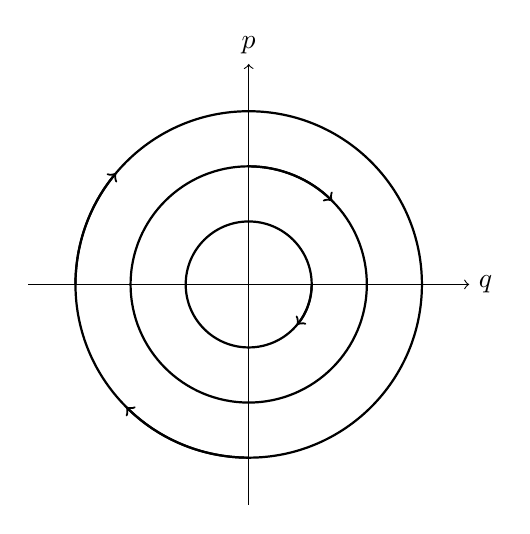
\begin{tikzpicture}[scale=1.0]
\draw[->] (-2.8,0) -- (2.8,0) node[right] {$q$};
\draw[->] (0,-2.8) -- (0,2.8) node[above] {$p$};

\draw[thick] (0,0) circle (0.8);
\draw[thick] (0,0) circle (1.5);
\draw[thick] (0,0) circle (2.2);

\draw[->,thick] (0.8,0) arc[start angle=0,end angle=-40,radius=0.8];
\draw[->,thick] (0,1.5) arc[start angle=90,end angle=45,radius=1.5];
\draw[->,thick] (-2.2,0) arc[start angle=180,end angle=140,radius=2.2];
\draw[->,thick] (0,-2.2) arc[start angle=-90,end angle=-135,radius=2.2];
\end{tikzpicture}
\caption{For the harmonic oscillator, constant energy means concentric circles in the \(p\)-\(q\) plane. The flow runs tangentially along the circles.}
\end{figure}

Here the geometry and the motion are especially simple. A point started on one circle stays on that circle forever. The phase portrait rotates rigidly, and because the oscillator has one fixed frequency, the whole picture has the character of a carousel.

\subsection{Question \& Answer}

\paragraph{Question.} How do the equations of motion differ from the constant-energy surface?

\paragraph{Answer.} The distinction is essential. The equation
\begin{equation}
H(q,p)=E
\end{equation}
defines a locus of allowed points in phase space. It is one equation among the phase-space coordinates. The equations of motion, by contrast, specify the velocity vector at each point:
\begin{equation}
(\dot q_i,\dot p_i).
\end{equation}
The constant-energy surface tells us where the motion must live. Hamilton's equations tell us how it moves along that surface.

The lecture makes this distinction explicit because the two ideas are easily conflated. For the harmonic oscillator, the circles are the constant-energy surfaces. The Hamiltonian flow is the motion around those circles. One is a constraint on position in phase space; the other is a law of motion.

\section{From One Phase Point to a Fluid of Phase Points}

Now the lecture makes a crucial change of scale. Instead of choosing one initial condition and following one phase point, we imagine all possible initial conditions at once. The phase plane is sprinkled with points. Every point is a possible state of the system, and every point moves according to the same Hamiltonian rules.

To visualize that, Susskind asks us to think of an imaginary fluid, or better, a dust so fine that it may as well be a fluid. This is not a real material fluid. It is a picture of the collection of states. One starts the clock, and the whole dust moves through phase space.

\begin{definition}
The phase-space velocity field is the vector field whose components are all the phase-space time derivatives:
\begin{equation}
\mathbf V
=
(\dot q_1,\dots,\dot q_n,\dot p_1,\dots,\dot p_n).
\end{equation}
For a single canonical pair we write
\begin{equation}
V_q=\dot q, \qquad V_p=\dot p.
\end{equation}
\end{definition}

The important point is that these components are determined entirely by the Hamiltonian. Once \(H\) is known, every point in phase space has an assigned velocity. In the time-independent case this is a stationary flow: what happens next depends only on where the point is, not on the absolute time at which it gets there.

For the harmonic oscillator the picture is especially simple. The entire sprinkling rotates rigidly. Points at smaller radius move more slowly in magnitude, but they go around in the same period, because the oscillator's frequency is independent of amplitude.

\begin{figure}[h]
\centering
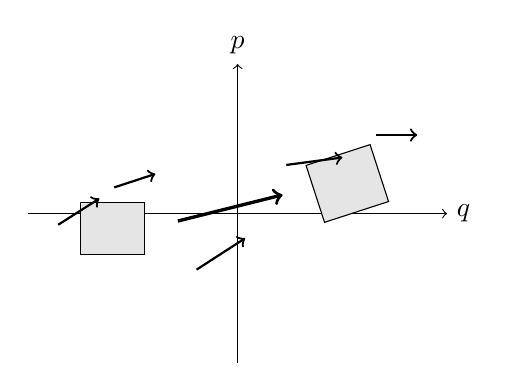
\begin{tikzpicture}[scale=0.95]
\draw[->] (-2.8,0) -- (2.8,0) node[right] {$q$};
\draw[->] (0,-2.0) -- (0,2.0) node[above] {$p$};

\filldraw[fill=gray!20,draw=black] (-2.1,-0.55) rectangle (-1.25,0.15);
\filldraw[fill=gray!20,draw=black,rotate around={18:(1.45,0.45)}] (1.0,0.0) rectangle (1.9,0.8);

\foreach \x/\y/\u/\v in {-2.4/-0.15/0.55/0.35,-1.65/0.35/0.55/0.18,-0.55/-0.75/0.65/0.42,0.65/0.65/0.75/0.10,1.85/1.05/0.55/0.00}
{
\draw[->,thick] (\x,\y) -- ++(\u,\v);
}

\draw[->,very thick] (-0.8,-0.1) -- (0.6,0.25);
\end{tikzpicture}
\caption{A patch of phase space transported by the phase-space velocity field. The picture is mnemonic only: the points are states of the system, not material particles in ordinary space.}
\end{figure}

We have now arrived at the right object. Liouville's theorem is not merely a statement about one orbit staying on one energy contour. It is a statement about the motion of an extended patch of phase space under the Hamiltonian flow.

\subsection{Question \& Answer}

\paragraph{Question.} What is this fluid, exactly?

\paragraph{Answer.} It is only a visualization. Each point is a state of the system, not a particle of the original mechanical model. If the language of fluid helps, we use it. If it does not, we can forget the fluid and phrase everything directly in terms of regions of phase space: take a patch, evolve every point in it, and ask whether its phase-space volume changes.

This is exactly how the lecture resolves the question. The fluid picture is useful, but the actual content of the theorem is about states and regions in phase space.

\section{Compressibility, Divergence, and the Setup for Liouville}

The question is now sharpened: is the phase-space flow compressible or incompressible?

The lecture builds the answer slowly, beginning with one dimension. A one-dimensional fluid has a velocity \(v(x)\). If \(v\) gets larger as we move to the right, neighboring points separate. If \(v\) gets smaller, neighboring points bunch together. Thus in one dimension the incompressible condition is simply
\begin{equation}
\frac{dv}{dx}=0.
\end{equation}
Positive \(dv/dx\) means stretching; negative \(dv/dx\) means compression.

There are two equivalent ways to think about this. We may follow a moving little segment of the fluid and ask whether its length changes. Or we may stand still and watch fluid pass through a fixed region, demanding that as much enters as leaves. The lecture insists on both pictures, because the second one will connect directly to the old reversible arrow diagrams.

\begin{figure}[h]
\centering
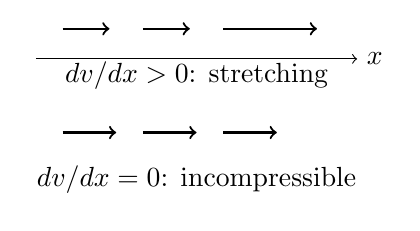
\begin{tikzpicture}[scale=0.85]
\draw[->] (-2.4,0) -- (2.4,0) node[right] {$x$};

\draw[->,thick] (-2.0,0.45) -- (-1.3,0.45);
\draw[->,thick] (-0.8,0.45) -- (-0.1,0.45);
\draw[->,thick] (0.4,0.45) -- (1.8,0.45);
\node at (0,-0.25) {$dv/dx>0$: stretching};

\draw[->,thick] (-2.0,-1.1) -- (-1.2,-1.1);
\draw[->,thick] (-0.8,-1.1) -- (0.0,-1.1);
\draw[->,thick] (0.4,-1.1) -- (1.2,-1.1);
\node at (0,-1.8) {$dv/dx=0$: incompressible};
\end{tikzpicture}
\hspace{1.0cm}
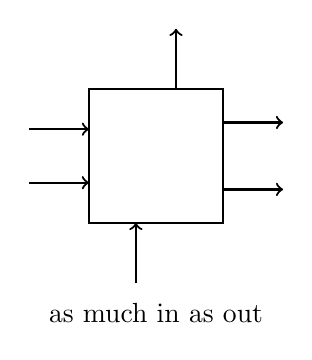
\begin{tikzpicture}[scale=0.85]
\draw[thick] (0,0) rectangle (2.0,2.0);

\draw[->,thick] (-0.9,0.6) -- (0,0.6);
\draw[->,thick] (-0.9,1.4) -- (0,1.4);

\draw[->,thick] (2.0,0.5) -- (2.9,0.5);
\draw[->,thick] (2.0,1.5) -- (2.9,1.5);

\draw[->,thick] (0.7,-0.9) -- (0.7,0);
\draw[->,thick] (1.3,2.0) -- (1.3,2.9);

\node at (1.0,-1.35) {as much in as out};
\end{tikzpicture}
\caption{Two equivalent pictures of incompressibility. Left: in one dimension a varying velocity field stretches or compresses neighboring points. Right: in higher dimensions one asks whether a fixed box has equal inflow and outflow.}
\end{figure}

In higher dimensions one must be more careful. A region may stretch in one direction and compress in another while preserving total volume. So we do not require
\(\partial V_x/\partial x=0\) by itself. We require instead that the sum of the same-coordinate derivatives vanish.

\begin{definition}
For a vector field \(\mathbf V=(V_x,V_y,V_z)\), the divergence is
\begin{equation}
\nabla\cdot\mathbf V
=
\frac{\partial V_x}{\partial x}
+
\frac{\partial V_y}{\partial y}
+
\frac{\partial V_z}{\partial z}.
\end{equation}
Incompressibility means
\begin{equation}
\nabla\cdot\mathbf V=0.
\end{equation}
\end{definition}

The lecture then translates this directly to phase space. For one canonical pair \((q,p)\) the relevant divergence is
\begin{equation}
\frac{\partial V_p}{\partial p}+\frac{\partial V_q}{\partial q}.
\end{equation}
The first term tells us about bunching in the \(p\)-direction; the second tells us about bunching in the \(q\)-direction.

At this point Susskind deliberately abandons the fluid notation for a moment and returns to the very first lecture. There the reversible discrete laws had one arrow in and one arrow out at each state. The irreversible laws had sinks. The new claim is that incompressibility of the phase-space flow is the continuous version of the first picture.

\begin{figure}[h]
\centering
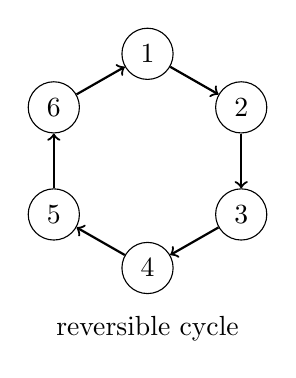
\begin{tikzpicture}[scale=0.85]
\foreach \x/\y/\name in {0/1.6/1,1.4/0.8/2,1.4/-0.8/3,0/-1.6/4,-1.4/-0.8/5,-1.4/0.8/6}
{
\node[circle,draw,minimum size=0.65cm] (\name) at (\x,\y) {\name};
}
\draw[->,thick] (1) -- (2);
\draw[->,thick] (2) -- (3);
\draw[->,thick] (3) -- (4);
\draw[->,thick] (4) -- (5);
\draw[->,thick] (5) -- (6);
\draw[->,thick] (6) -- (1);
\node at (0,-2.5) {reversible cycle};
\end{tikzpicture}
\hspace{1.2cm}
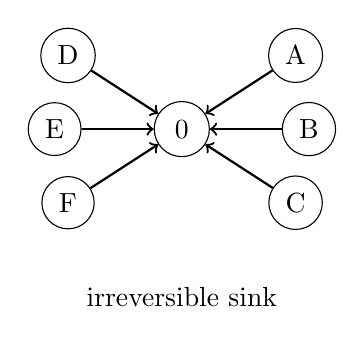
\begin{tikzpicture}[scale=0.85]
\node[circle,draw,minimum size=0.7cm] (c) at (0,0) {0};
\foreach \x/\y/\name in {1.7/1.1/A,1.9/0/B,1.7/-1.1/C,-1.7/1.1/D,-1.9/0/E,-1.7/-1.1/F}
{
\node[circle,draw,minimum size=0.65cm] (\name) at (\x,\y) {\name};
\draw[->,thick] (\name) -- (c);
}
\node at (0,-2.5) {irreversible sink};
\end{tikzpicture}
\caption{The old discrete pictures reappear in continuous form. Liouville's theorem will say that Hamiltonian flow is the analog of the reversible case, not the sink.}
\end{figure}

Now the question can be asked cleanly. If the velocity field in phase space is built from Hamilton's equations, is its divergence zero? Equivalently: if we take a small volume of phase space and follow it in time, does it keep the same volume?

\section{Liouville's Theorem}

Only after all of that preparation does the theorem itself appear.

\begin{theorem}[Liouville's theorem]
For Hamiltonian motion, the phase-space velocity field is incompressible. Equivalently, the divergence of the phase-space flow vanishes, and any patch of phase space preserves its volume under time evolution.
\end{theorem}

\begin{proof}
Let us begin with one canonical pair \((q,p)\). Define the phase-space velocity components by
\begin{equation}
V_p=\dot p, \qquad V_q=\dot q.
\end{equation}
Then the divergence is
\begin{equation}
\frac{\partial V_p}{\partial p}+\frac{\partial V_q}{\partial q}.
\end{equation}
Now substitute Hamilton's equations:
\begin{equation}
V_p=-\frac{\partial H}{\partial q}, \qquad V_q=\frac{\partial H}{\partial p}.
\end{equation}
Therefore
\begin{align}
\frac{\partial V_p}{\partial p}+\frac{\partial V_q}{\partial q}
&=
\frac{\partial}{\partial p}\!\left(-\frac{\partial H}{\partial q}\right)
+
\frac{\partial}{\partial q}\!\left(\frac{\partial H}{\partial p}\right) \\
&=
-\frac{\partial^2 H}{\partial p\,\partial q}
+
\frac{\partial^2 H}{\partial q\,\partial p}.
\end{align}
For a smooth function of independent variables, the mixed partial derivatives commute:
\begin{equation}
\frac{\partial^2 H}{\partial p\,\partial q}
=
\frac{\partial^2 H}{\partial q\,\partial p}.
\end{equation}
Hence
\begin{equation}
\frac{\partial V_p}{\partial p}+\frac{\partial V_q}{\partial q}=0.
\end{equation}

For many degrees of freedom, exactly the same cancellation occurs pair by pair:
\begin{equation}
\sum_i\left(
\frac{\partial \dot p_i}{\partial p_i}
+
\frac{\partial \dot q_i}{\partial q_i}
\right)=0.
\end{equation}
So the full Hamiltonian flow is incompressible.
\end{proof}

The lecture does not treat the commutation of mixed partial derivatives as a mere black-box theorem. It pauses to give the rectangle argument: the mixed second derivative is a difference of horizontal differences or a difference of vertical differences, and the two constructions lead to the same combination.

\begin{figure}[h]
\centering
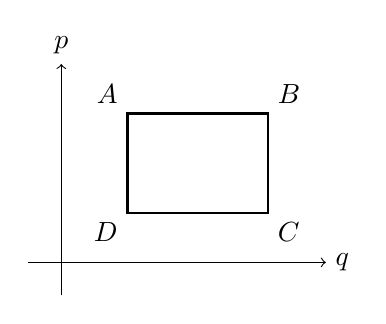
\begin{tikzpicture}[scale=1.05]
\draw[->] (-0.4,0) -- (3.2,0) node[right] {$q$};
\draw[->] (0,-0.4) -- (0,2.4) node[above] {$p$};
\draw[thick] (0.8,0.6) rectangle (2.5,1.8);
\node[above left] at (0.8,1.8) {$A$};
\node[above right] at (2.5,1.8) {$B$};
\node[below right] at (2.5,0.6) {$C$};
\node[below left] at (0.8,0.6) {$D$};
\end{tikzpicture}
\caption{The finite-difference rectangle behind the lecture's side-proof. The combination \(F(B)+F(D)-F(A)-F(C)\) appears whichever order of differentiation is taken.}
\end{figure}

The theorem is often summarized as conservation of phase-space volume, but the lecture phrases it both ways. We may follow a patch and say its volume does not change, or we may fix a small region and say that as much flow enters as leaves. The two statements are equivalent.

\begin{remark}
The cancellation happens pairwise in each canonical pair. In that sense Hamiltonian flow is not merely incompressible in some accidental way; it is a special kind of incompressible flow built out of conjugate directions.
\end{remark}

\subsection{Question \& Answer}

\paragraph{Question.} Why does Liouville's theorem survive even when the Hamiltonian depends explicitly on time, whereas conservation of energy did not?

\paragraph{Answer.} The two questions are different. Conservation of energy asks whether \(H\) itself remains constant along the motion, and that is why \(\partial H/\partial t\) appears in
\begin{equation}
\frac{dH}{dt}=\frac{\partial H}{\partial t}.
\end{equation}
Liouville's theorem asks instead about the divergence of the velocity field. In the one-pair case the relevant combination is
\begin{equation}
\frac{\partial}{\partial p}\!\left(-\frac{\partial H}{\partial q}\right)
+
\frac{\partial}{\partial q}\!\left(\frac{\partial H}{\partial p}\right),
\end{equation}
and those terms still cancel even if \(H\) also depends on \(t\). The theorem is about the geometry of Hamiltonian flow in phase space, not about whether the Hamiltonian is numerically constant along that flow.

\section{Consequences, Counterexamples, and Outlook}

Now we interpret the theorem, and here the lecture becomes careful. There are really two different statements on the table. One is that a single orbit remains on a constant-energy surface. The other is that a finite patch of phase space preserves its volume. These are not the same statement. A patch may cut across many different energy surfaces and still evolve with fixed volume.

The harmonic oscillator is deceptive because it does both things in the cleanest possible way. An orbit stays on a circle, and a small region rotates rigidly, preserving both area and shape. But Liouville's theorem promises only the first part of that second statement: it preserves volume, not shape. The lecture is emphatic on this point.

It also draws broader consequences. Distinct phase points do not coalesce. A region may be stretched into a long filament, but it does not collapse into a smaller-volume set. The lecture goes further and treats topology preservation as an informal companion claim: a blob may become extraordinarily thin, but it does not pinch off into disconnected pieces, because each phase point has a unique forward direction determined by the Hamiltonian.

\begin{remark}
The lecture also stresses what Liouville's theorem does \emph{not} preserve. In general it does not preserve shape, and it certainly does not preserve angles. The harmonic oscillator is exceptional in that its flow is a rigid rotation.
\end{remark}

A brief application then appears. If a gas expands in ordinary \(q\)-space, the phase-space volume can remain constant only if the momentum distribution contracts. That is why the momenta move toward zero and the gas cools. The lecture mentions the expanding universe as an analogy, but keeps the real point local: expansion in one set of directions must be balanced by contraction in the conjugate directions if the total phase-space volume is to stay fixed.

Now comes the lecture's main stress test.

\begin{figure}[h]
\centering

\includegraphics[width=0.58\textwidth]{lecture_07_figure_03.png}
\caption{The board at the start of the \(H=pq\) example: the Hamiltonian is written, and the first component of the phase-space velocity field is extracted from it.}
\end{figure}

Take
\begin{equation}
H=pq.
\end{equation}
The first visible board equation is
\begin{equation}
V_p=\dot p=-\frac{\partial H}{\partial q}.
\end{equation}
Completing the calculation gives
\begin{equation}
\dot p=-p,
\qquad
\dot q=\frac{\partial H}{\partial p}=q.
\end{equation}
So the motion contracts exponentially in the \(p\)-direction and expands exponentially in the \(q\)-direction. Indeed,
\begin{equation}
p(t)=p_0 e^{-t},
\qquad
q(t)=q_0 e^{t}.
\end{equation}
A small square patch is squeezed one way and stretched the other way. The result is dramatic shape change with no loss of area.

The lecture insists on checking the divergence explicitly:
\begin{equation}
\frac{\partial V_p}{\partial p}+\frac{\partial V_q}{\partial q}
=
(-1)+(1)=0.
\end{equation}
So the area is preserved even while the shape changes violently.

\begin{remark}
The product \(pq\) has the units of action, and so does a phase-space area element. But Liouville's theorem is not the conservation of action. The theorem is about conservation of phase-space volume.
\end{remark}

\begin{figure}[h]
\centering
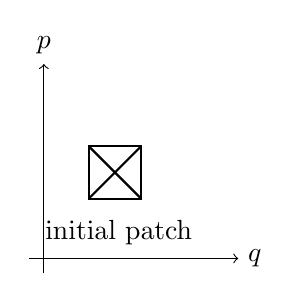
\begin{tikzpicture}[scale=0.95]
\draw[->] (-0.2,0) -- (2.6,0) node[right] {$q$};
\draw[->] (0,-0.2) -- (0,2.6) node[above] {$p$};
\draw[thick] (0.6,0.8) rectangle (1.3,1.5);
\draw[thick] (0.6,0.8) -- (1.3,1.5);
\draw[thick] (0.6,1.5) -- (1.3,0.8);
\node at (1.0,0.35) {initial patch};
\end{tikzpicture}
\hspace{1.0cm}
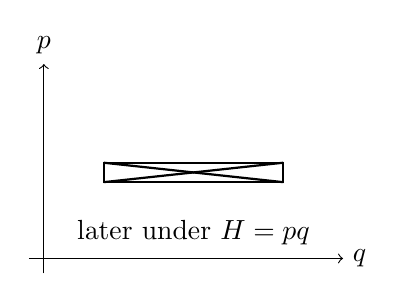
\begin{tikzpicture}[scale=0.95]
\draw[->] (-0.2,0) -- (4.0,0) node[right] {$q$};
\draw[->] (0,-0.2) -- (0,2.6) node[above] {$p$};
\draw[thick] (0.8,1.02) rectangle (3.2,1.28);
\draw[thick] (0.8,1.02) -- (3.2,1.28);
\draw[thick] (0.8,1.28) -- (3.2,1.02);
\node at (2.0,0.35) {later under \(H=pq\)};
\end{tikzpicture}

\vspace{0.8cm}

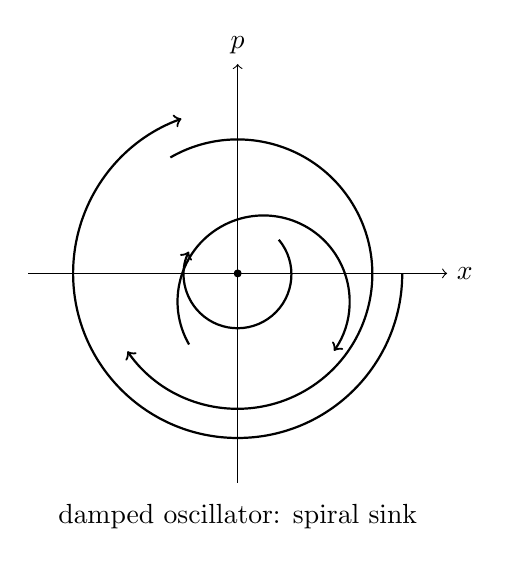
\begin{tikzpicture}[scale=0.95]
\draw[->] (-2.8,0) -- (2.8,0) node[right] {$x$};
\draw[->] (0,-2.8) -- (0,2.8) node[above] {$p$};
\draw[->,thick] (2.2,0) arc[start angle=0,end angle=-250,radius=2.2];
\draw[->,thick] (-0.9,1.55) arc[start angle=120,end angle=-145,radius=1.8];
\draw[->,thick] (-0.65,-0.95) arc[start angle=210,end angle=-35,radius=1.15];
\draw[->,thick] (0.55,0.45) arc[start angle=40,end angle=-205,radius=0.72];
\filldraw (0,0) circle (1.3pt);
\node at (0,-3.25) {damped oscillator: spiral sink};
\end{tikzpicture}
\caption{Top: under \(H=pq\), a patch of phase space is stretched in \(q\) and squeezed in \(p\), preserving area while changing both shape and angles. Bottom: the damped oscillator contracts toward the origin and therefore fails to satisfy Liouville's theorem.}
\end{figure}

To see what fails outside Hamiltonian mechanics, the lecture turns to the damped harmonic oscillator,
\begin{equation}
m\ddot x=-kx-c\dot x.
\end{equation}
If we define
\begin{equation}
p=m\dot x,
\end{equation}
then the phase-space equations become
\begin{equation}
\dot x=\frac{p}{m},
\qquad
\dot p=-kx-\frac{c}{m}p.
\end{equation}
The divergence is now
\begin{equation}
\frac{\partial \dot x}{\partial x}+\frac{\partial \dot p}{\partial p}
=
0-\frac{c}{m}<0.
\end{equation}
So the phase-space flow converges. A patch shrinks toward the origin, and the origin acts as a sink.

This example also clarifies a point made explicitly in the lecture: Newton's equation \(F=ma\) is broader than Hamiltonian mechanics. Dissipative forces such as viscous drag can certainly appear in Newtonian form, but they do not come from a potential, and therefore they do not fit into the Hamiltonian structure used here.

The damped oscillator is then described as the closest classical continuous analog of information loss. Strictly speaking, in a continuum one can still imagine infinite precision and integrate the equations backward. But what is no longer preserved is the finite phase-space volume carried by a little cell of initial conditions. Those cells lose their integrity and are compressed into smaller and smaller regions.

\subsection{Question \& Answer}

\paragraph{Question.} Can divergence vanish without a Hamiltonian?

\paragraph{Answer.} Yes. Hamiltonian flow is sufficient for zero divergence, but not necessary. The lecture gives the example of an ordinary incompressible fluid in three spatial dimensions. Its velocity field can have zero divergence, but it does not come from a Hamiltonian of the present kind, because Hamiltonian phase space is always even-dimensional. Thus the logic is one-way:
\begin{equation}
\text{Hamiltonian flow}
\Longrightarrow
\text{incompressible phase-space flow},
\end{equation}
but not conversely.

The lecture closes with a bridge to the next formal repackaging. If \(F(q,p)\) is any function on phase space, then
\begin{equation}
\frac{dF}{dt}
=
\sum_i\left(
\frac{\partial F}{\partial q_i}\dot q_i
+
\frac{\partial F}{\partial p_i}\dot p_i
\right)
=
\sum_i\left(
\frac{\partial F}{\partial q_i}\frac{\partial H}{\partial p_i}
-
\frac{\partial F}{\partial p_i}\frac{\partial H}{\partial q_i}
\right).
\end{equation}
Poisson gives a name to that antisymmetric combination:
\begin{equation}
\{f,g\}
=
\sum_i\left(
\frac{\partial f}{\partial q_i}\frac{\partial g}{\partial p_i}
-
\frac{\partial f}{\partial p_i}\frac{\partial g}{\partial q_i}
\right),
\end{equation}
so that, in particular,
\begin{equation}
\frac{dF}{dt}=\{F,H\}.
\end{equation}
The lecture does not develop the bracket further here. It is only a bridge. The real work of this chapter was to build the language in which Liouville's theorem becomes visible.

\section{Summary}

Liouville's theorem is the classical-mechanical statement that Hamiltonian flow preserves phase-space volume. The lecture reaches it deliberately: first Hamilton's equations, then conservation of the Hamiltonian, then constant-energy surfaces, then the fluid picture in phase space, then divergence, and only then the proof. The theorem is the continuous counterpart of the old reversible arrow diagrams: as much flows in as flows out.

The interpretation matters as much as the proof. A single orbit staying on a fixed energy surface is one statement. A whole patch of phase space preserving its volume is another. The harmonic oscillator makes both statements look rigid and simple, but the \(H=pq\) example shows the more general truth: volume is preserved while shape may change drastically. The damped oscillator, by contrast, produces a genuine sink and lies outside Hamiltonian mechanics. That is the boundary the lecture wanted us to see.